\scanpage{96}
\diagram{\begin{array}{ccccc}
\mathring P^{\unsure{+|\#}}&\subset&P^{\unsure{+|\#}}&\subset&\overline{P^{\unsure{+|\#}}}\\
\cup&&&&\cup\\
\mathring Q^{\unsure{+|\#}}&\subset&Q^+&=&\overline{Q^{\unsure{+|\#}}}\\
\cup&&&&\cup\\
\mathring{\overline R}&=&R&\subset&\overline R
\end{array}}

\[\boxed{\mathring Q^{\unsure{+|\#}}\subset P^{\unsure{+|\#}}}\quad
\text{d'où}\quad Q^{\unsure{+|\#}}=\overline{Q^{\unsure{+|\#}}}\subset\overline{P^{\unsure{+|\#}}}\]
\margin{\uline{Prop} de \uline{\unsure{Cauchy|Castel.}}}
\[\left(\text{donc }\mathring Q^{\unsure{+|\#}}\subset\mathring{\overline{P^{\unsure{+|\#}}}}=\mathring P^{\unsure{+|\#}}\right)\]
d'où par polarité, comme $Q^+=Q^{+0}$
\[\overline{P^{\unsure{+|\#}}}^{\,0}=P^{\unsure{+|\#}0}\subset Q^{\unsure{+|\#}}.\]

\[P^+\ni x\quad\Longleftrightarrow\quad\exists\ C>0,\ \inserted{n>0}\ \text{tel que }\gamma(C)=nx\quad\Longleftrightarrow\quad
\figure{\begin{tikzpicture}[baseline=(condition.base)]\node[draw,rounded corners,inner sep=4pt] (condition) {$\begin{gathered}\deleted{\unsure{\text{si }x\text{ est}}}\\\ell(nx)\geq2\text{ si }n\text{ grand}\end{gathered}$};\end{tikzpicture}}\]

\[Q^+\ni x\quad\Longleftrightarrow\quad\begin{cases}x^2\geq0\\x.a\geq0\end{cases},\qquad
\mathring Q^{\unsure{+|\#}}\ni x\quad\Longleftrightarrow\quad x^2>0,\ x.a\geq0\]
\margin{$[a$ choisi dans $\unsure{\mathring Q^{+}|Q^+}]$ p.ex $a$ dans $R\ ]$}
\[R\ni x\quad\Longleftrightarrow\quad\exists\ C\ \uline{\text{ample}},\ n>0,\ \text{tel que }\gamma(C)=nx\]
\hrulefill
\[\boxed{x\in R\quad\underset{\substack{\vert\\\text{th. de}\\\text{Nakai}}}{\Longleftrightarrow}\quad\deleted{\unsure{x\in P}}\quad x.P>0\quad\text{et}\quad x^2>0}\]
\figure{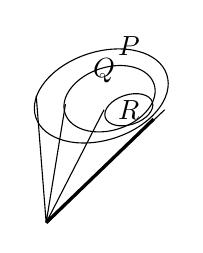
\begin{tikzpicture}[x=.7cm,y=.7cm]
\coordinate (v) at (0,0);
\draw[rotate around={18:(1,2.3)}] (1,2.3) ellipse (1.25 and .8);
\draw[rotate around={18:(1.15,2.25)}] (1.15,2.25) ellipse (.85 and .57);
\draw[rotate around={18:(1.5,2.05)}] (1.5,2.05) ellipse (.45 and .27);
\draw (v)--(-.18,2.3) (v)--(.35,2.15) (v)--(1.05,2.05) (v)--(2.15,2.05);
\draw[very thick] (v)--(1.95,1.88);
\node at (1.5,3.2) {$P$};\node at (1.05,2.75) {$Q$};\node at (1.5,2.05) {$R$};
\end{tikzpicture}}
\[\overline R\subset\unsure{\overline P^{\,0}|P^0}\cap Q=P^0=\overline P^{\,0},\quad\deleted{\unsure{a}}\quad\text{d'où}\]
\deleted{$\boxed{\unsure{\overline R\subset R}}\quad\unsure{\text{donc }P^0}$}
\[R=\mathring{\overline R}\subset\mathring{\overline{P^0}},\quad\text{je dis qu'on a \uline{égalité}, car}\]
\[\mathring{P^0}\subset\mathring Q\quad\text{et on applique le critère de Nakai}\]
\diagram{\boxed{\begin{array}{ccc|c}
R=\mathring{\overline R}&=&\mathring{P^0}\subset&\mathring Q\\
\overline R=P^0&=&\overline P^{\,0}\subset&Q
\end{array}}}

\uline{Question}\quad $xP>0\ \overset{?}{\Longrightarrow}\ x\in R$

Par Nakai, il reste à voir si $\uline{x^2>0}$

\deleted{Donc} $x^2\geq0$, il reste à voir $x^2\neq0$

On peut supposer que $x$ provient de $D$ div. tel que $D^2=0$. Mais alors $\chi(\mathcal L(nD))=\chi(X)+n\chi(D)$ et $h^0(\mathcal L(nD))\geq\chi(\mathcal L(nD))$ pour $n$ grand par Mumford, on doit donc avoir $\chi(D)\unsure{<|\leq}0$
\margin{95}
